\begin{DEFINITION}
    \p
    به هر عبارتی که بر حسب تابعی از عبارت‌های قبلی بیان بشود یک
    \FOCUSEDON{رابطه} 
    \FOCUSEDON{بازگشتی}  
     گفته می‌شود.
\end{DEFINITION}

\begin{PROBLEM}
    \p
    تعداد حالت‌های پرکردن یک جدول 
    $2\times n$
    با کاشی‌های
    $2\times 1$
    را به صورت یک رابطه بازگشتی 
    $f(n)$
    بیابید.
    چرخاندن کاشی‌ها مجاز است.
    \begin{center}
        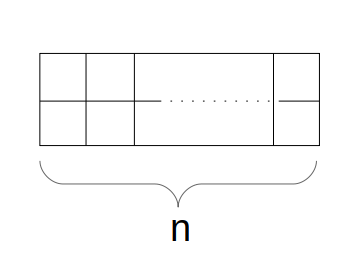
\includegraphics[totalheight=4cm]{im1.png}
        \end{center}
    \SOLUTION{
        \p
        دو حالت برای قرار دادن کاشی در خانه اول از سمت چپ وجود دارد:
        \begin{itemize}
            \item 
        اگر کاشی اول را به صورت عمودی قرار بدهیم, بقیه مسئله تبدیل به کاشی کاری یک جدول
            $2\times n-1$
        می‌شود.
        \begin{center}
            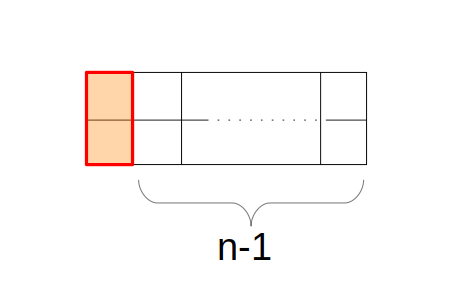
\includegraphics[totalheight=4cm]{im2.png}
            \end{center}
        \item 
        اگر کاشی اول را به صورت افقی قرار بدهیم, باید پایین آن یک کاشی افقی دیگر قرار بدهیم و بقیه مسئله تبدیل به کاشی‌کاری یک جدول
        $2\times n-2$
        می‌شود.
        \begin{center}
            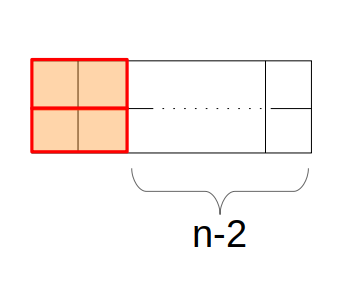
\includegraphics[totalheight=4cm]{im3.png}
            \end{center}
        \end{itemize}
        بنابراین طبق اصل جمع کل حالت‌ها برابر
        $f(n)=f(n-1)+f(n-2)$
        است.
        \p
        همانطور که در بخش دنباله‌های بازگشتی اشاره شد, لازم است که دو شرط اولیه برای این رابطه بازگشتی پیدا کنیم. بنابرین لازم است حالت
        $n=1$
        و
        $n=2$
        را به صورت دستی بررسی کنیم:
        $$f(1)=1$$
        \begin{center}
            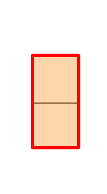
\includegraphics[totalheight=3cm]{im5.png}
            \end{center}
        $$f(2)=2$$
        \begin{center}
            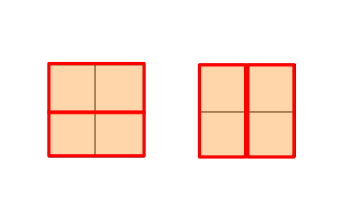
\includegraphics[totalheight=3cm]{im4.png}
            \end{center}
   
    }

 \end{PROBLEM}


\begin{DEFINITION}
    \FOCUSEDON{رابطه‌ بازگشتی خطی از درجه $k$}
    رابطه‌ای به فرم
   \[a_n=c_{1}a_{n-1}+c_{2}a_{n-2}+...+c_{k}a_{n-k}+F(n)\]
   است که
   $\forall{i}:c_i \in \mathbb{R} $
   و 
   $ c_k\neq 0$

\end{DEFINITION}


 \begin{DEFINITION}
    \p
    \FOCUSEDON{رابطه‌ بازگشتی خطی همگن از درجه $k$}
    رابطه‌ای به فرم
   \[a_n=c_{1}a_{n-1}+c_{2}a_{n-2}+...+c_{k}a_{n-k}\]
   است که
   $\forall{i}:c_i \in \mathbb{R} $
   و 
   $ c_k\neq 0$.


\end{DEFINITION}
